\chapter{Анализ спектральных данных}
\label{cha:ch_5}

Данная глава посвящена анализу экспериментальных данных, в результате которого планируется
получить подтверждение или опровержение согласования теоретических расчетов (см.~раздел~\ref{sec:link_ratio_and_TE})
с экспериментом, оценить осевое электрическое поле $E_z$ и электронную температуру $T_e$ для электронов, участвующих
в неупругих столкновениях, в возмущенном пылевыми частицами положительном столбе газового разряда
постоянного тока.
\section{Лабораторный журнал}

Как и было описано в разделе~\ref{sec:experiment} на борту МКС на научной аппаратуре «Плазменный~кристалл~-~4»
был проведен нужный космический эксперимент 4 июня 2015 года с 16:04:26 до 16:05:38. В результате которого были
получены видеофайлы «VM1-AVI-150604-160426.avi» (левая камера высокого разрешения CCD1),
«VM2-AVI-150604-160427.avi» (правая камера высокого разрешения CCD2), «VM3-AVI-150604-160428.avi» (общая камера наблюдения CCD3),
файл со спектральными данными «EAC\_Spectrum.dat», а также файл с логированием всех действий «PK4-particletrappingmanipulation.log».
Спектральные данные для первого спектра в эксперименте представлены в \hyperref[app:app1]{приложении А},
а логи за все время эксперимента приведены в \hyperref[app:app2]{приложении~Б}.

В ходе сопоставления полученных данных действительности и синхронизации всех каналов между собой, были сделаны
следующие лабораторные записи:

\begin{figure}[t]
    \centering
    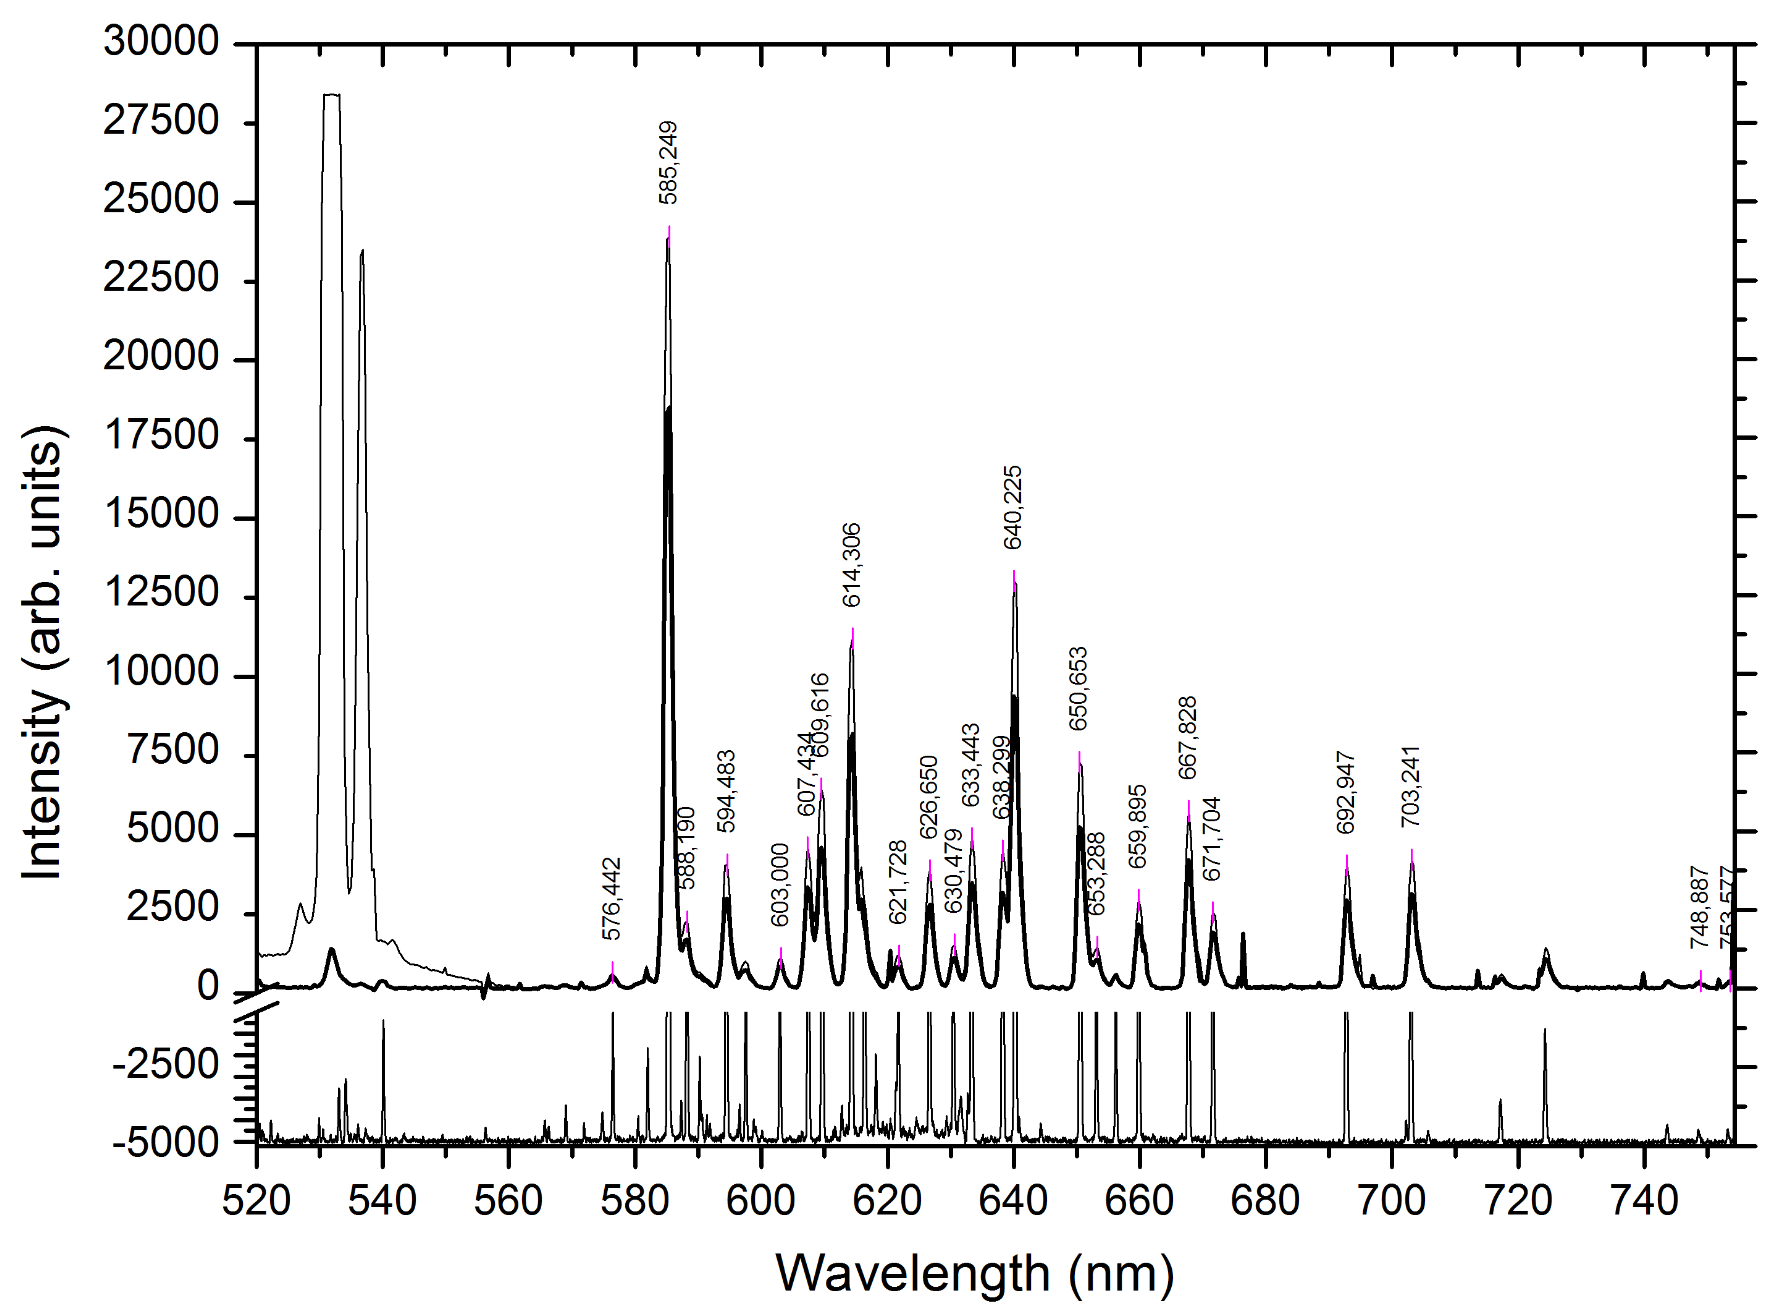
\includegraphics[width=16cm]{figures/main_spectrum}
    \caption{
        Наложенные спектры для трех конфигураций, усредненные и откалиброванные по длинам волн:
        жирной линией выделен спектр без пылевого облака; тонкой линией выделен спектр с пылевым облаком;
        ниже нуля достоверный спектр высокого разрешения атомарного неона.
    }
    \label{fig:main_spectrum}
\end{figure}

\begin{enumerate}
    \item Видео с левой камеры высокого разрешения CCD1:
    \begin{enumerate}
        \item отсутствие облака, время на видео: 0~--~33~с и 58~--~72~с;
        \item хорошая видимость облака, время на видео: 36~--~46~с;
    \end{enumerate}
    \item Видео с правой камеры высокого разрешения CCD2:
    \begin{enumerate}
        \item отсутствие облака, время на видео: 0~--~31~с и 59~--~71~с;
        \item хорошая видимость облака, время на видео: 35~--~53~с;
    \end{enumerate}
    \item Спектральные данные:
    \begin{enumerate}
        \item темновой ток, номера спектров: 52~--~55
        \item отсутствие облака, номера спектров: 888~--~895 и 903~--~904;
        \item хорошая видимость облака, номера спектров: 897~--~900;
    \end{enumerate}
    \item логи экспериментов не противоречат философии эксперимента: параметры разряда искусственно не менялись;
\end{enumerate}

\begin{figure}[t]
    \centering
    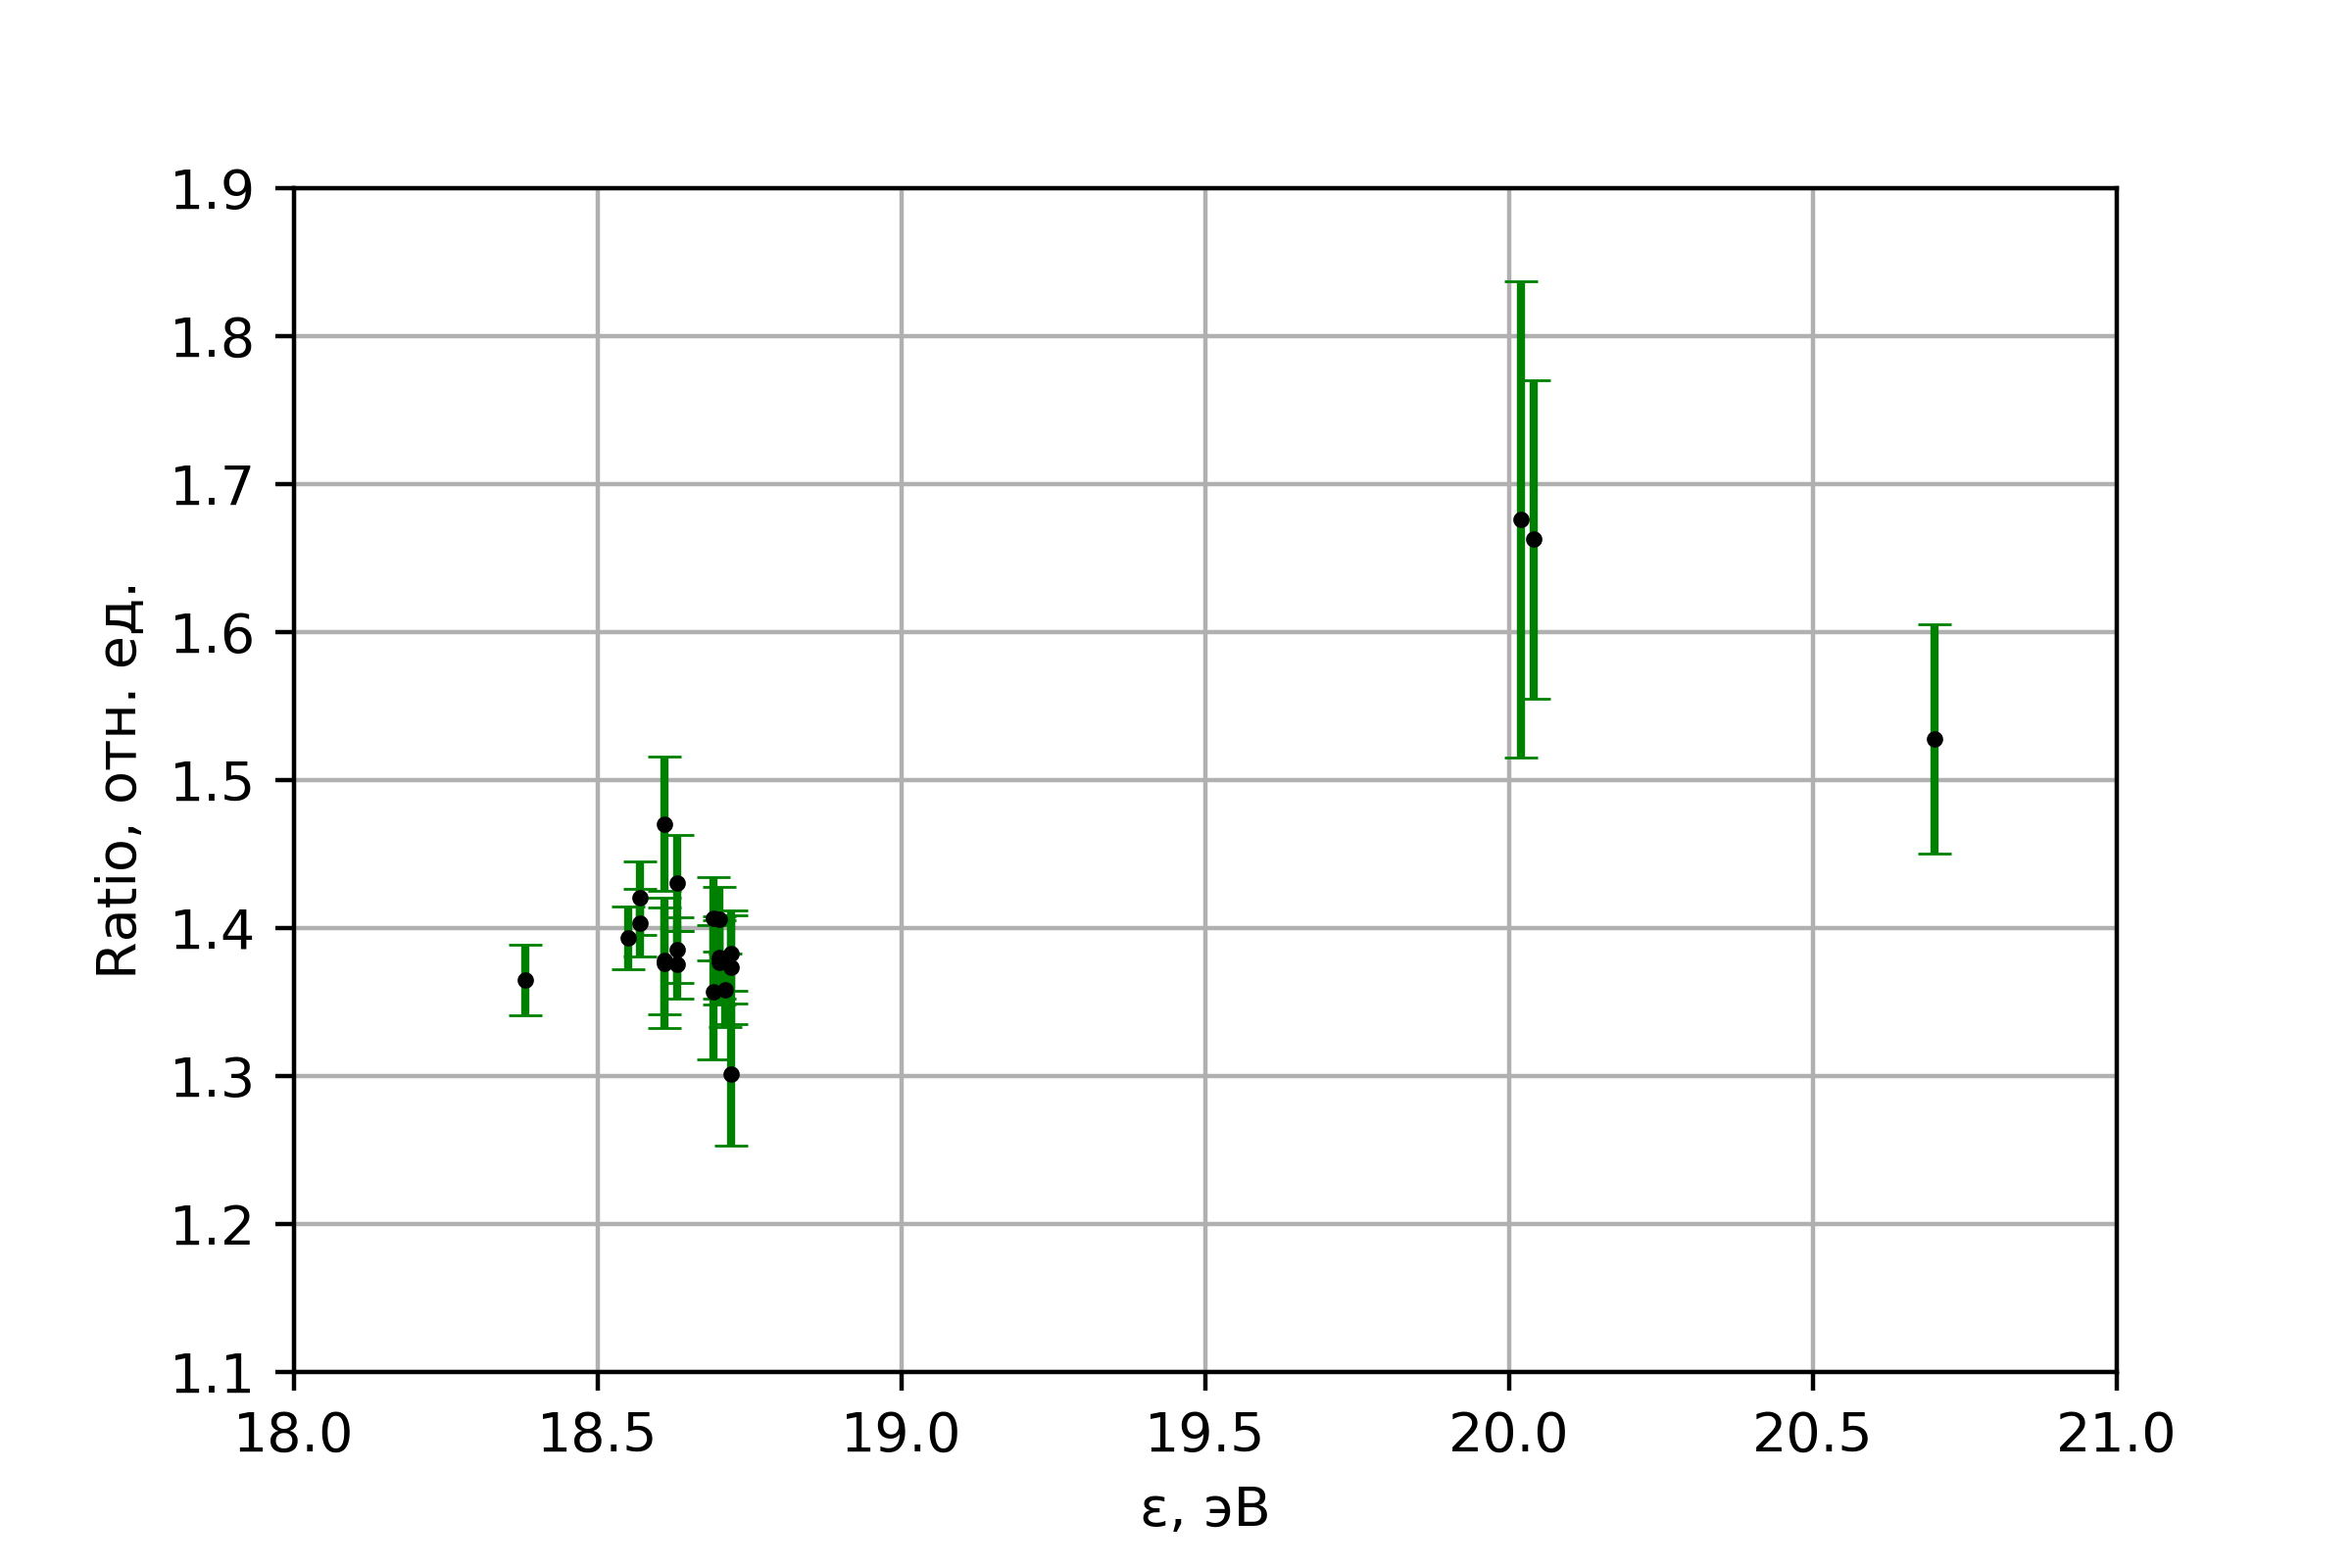
\includegraphics[width=16cm]{figures/experimental_ratio}
    \caption{Зависимость отношения интенсивностей спектральных линий неона в присутствии пылевого облака к отсутствию пылевого облака, полученного экспериментальным путем.}
    \label{fig:experimental_ratio}
\end{figure}

\section{Первичная обработка спектральных данных, наблюдение эффекта}

Для первичной обработки спектров, а именно для вычитания шумов и усреднения идеологически одинаковых спектров,
предлагается воспользоваться программой «Spectral~Analyzer~PK4», которая умеет обрабатывать спектры с НА~ПК-4 с учетом
среднеквадратичных погрешностей. Далее, были идентифицированы по длинам волн спектральные линии атомарного неона с помощью справочника~
\cite{Stritanov1966} и спектра неона, полученного с помощью спектрометра высокого разрешения МДР-12.
Для наглядности были наложены на один график
спектр невозмущенного состояния положительного столба газового разряда постоянного тока,
спектр возмущенного пылевым облаком положительного столба газового разряда постоянного тока и
спектр высокого разрешения для атомарных линий неона, а также отмечены идентифицированные линии~(см.~рисунок~\ref{fig:main_spectrum}).
Из данного рисунка следует отметить, что экспериментально наблюдается увеличение интенсивностей спектральных
линий при попадании пылевого облака в положительный столб газового разряда постоянного тока,
а также появление 532~нм сильного излучения, которое получено за счет рассеяния на пылевых частицах
532~нм лазерного ножа, используемого для подсветки.
\begin{figure}[t]
  \centering
  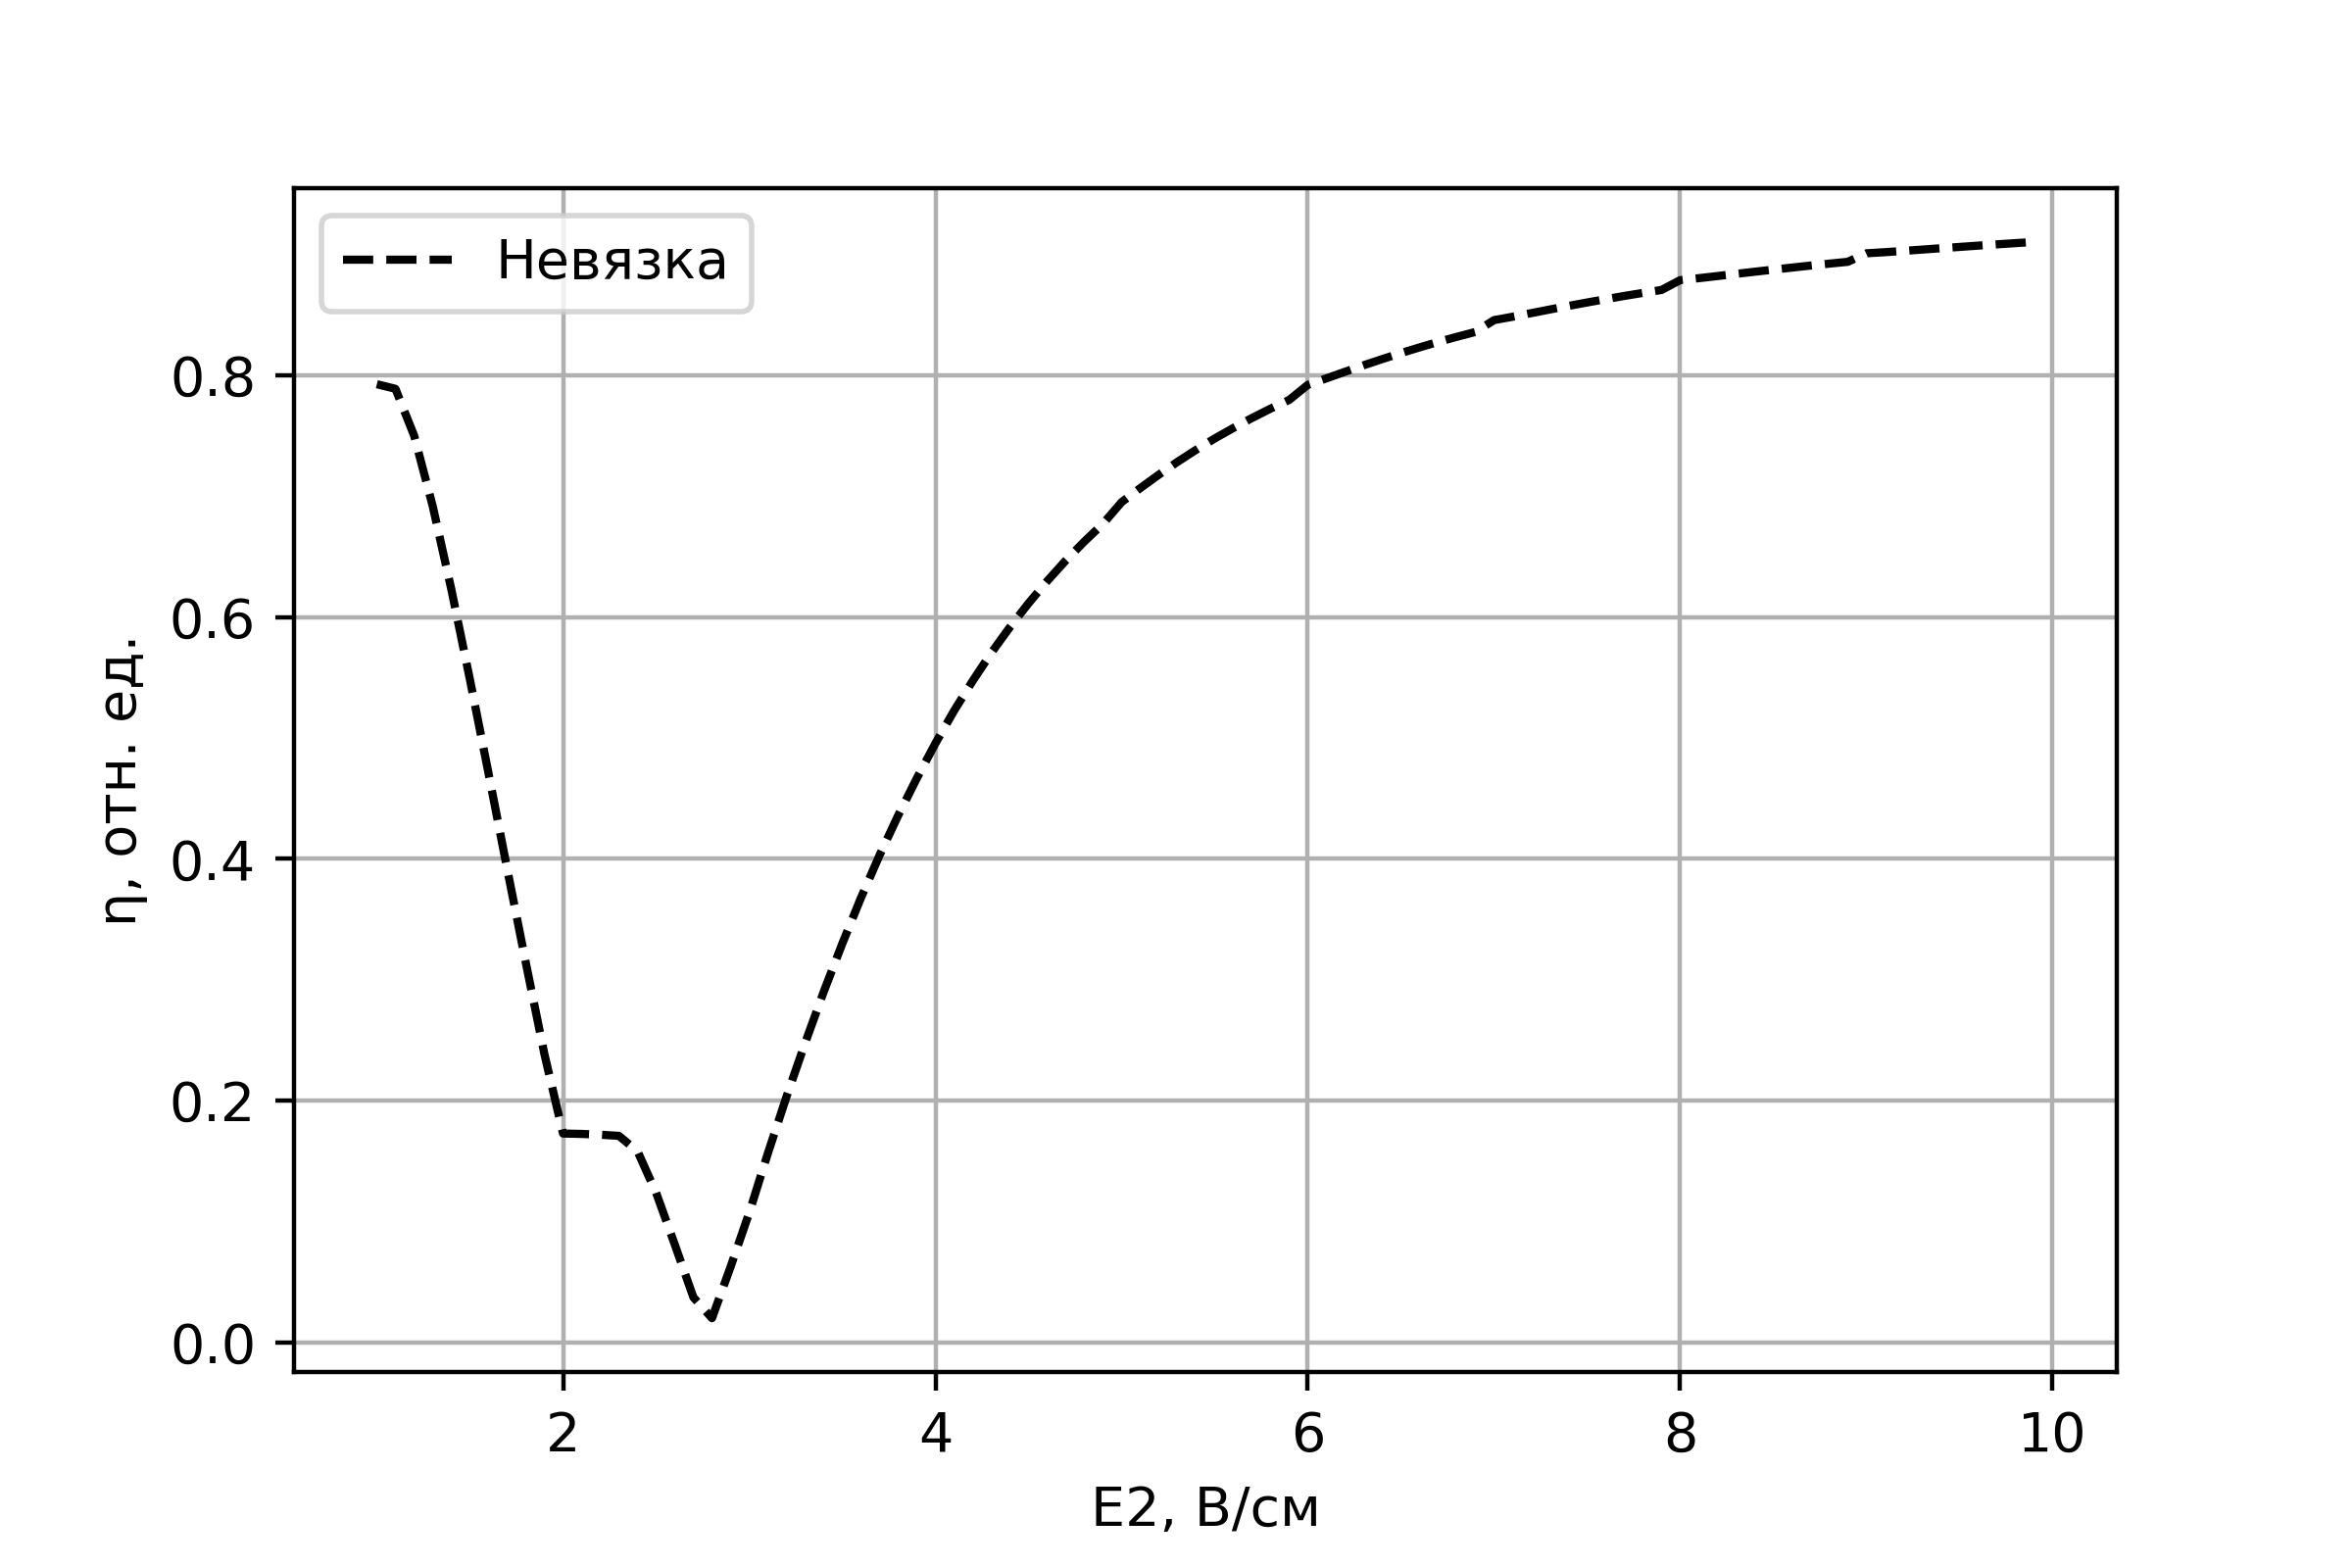
\includegraphics[width=16cm]{figures/discrepancy}
  \caption{Невязка аппроксимации расчетных отношений интенсивностей к отношениям интенсивностей, полученных из
  экспериментальных спектров, в зависимости от осевого электрического поля положительного столба газового разряда постоянного тока.}
  \label{fig:discrepancy}
\end{figure}

Сопоставив каждой спектральной линии энергию возбужденного состояния согласно справочнику~\cite{Stritanov1966},
можно построить зависимость отношения спектральных интенсивностей от энергии возбужденного состояния (см.~рисунок~\ref{fig:experimental_ratio}).
Основные характеристики атомарных линий неона, полученных в ходе обработки данных, можно найти в \hyperref[app:app3]{приложении В}.

\section{Оценка электронной температуры}
\begin{figure}[t]
  \centering
  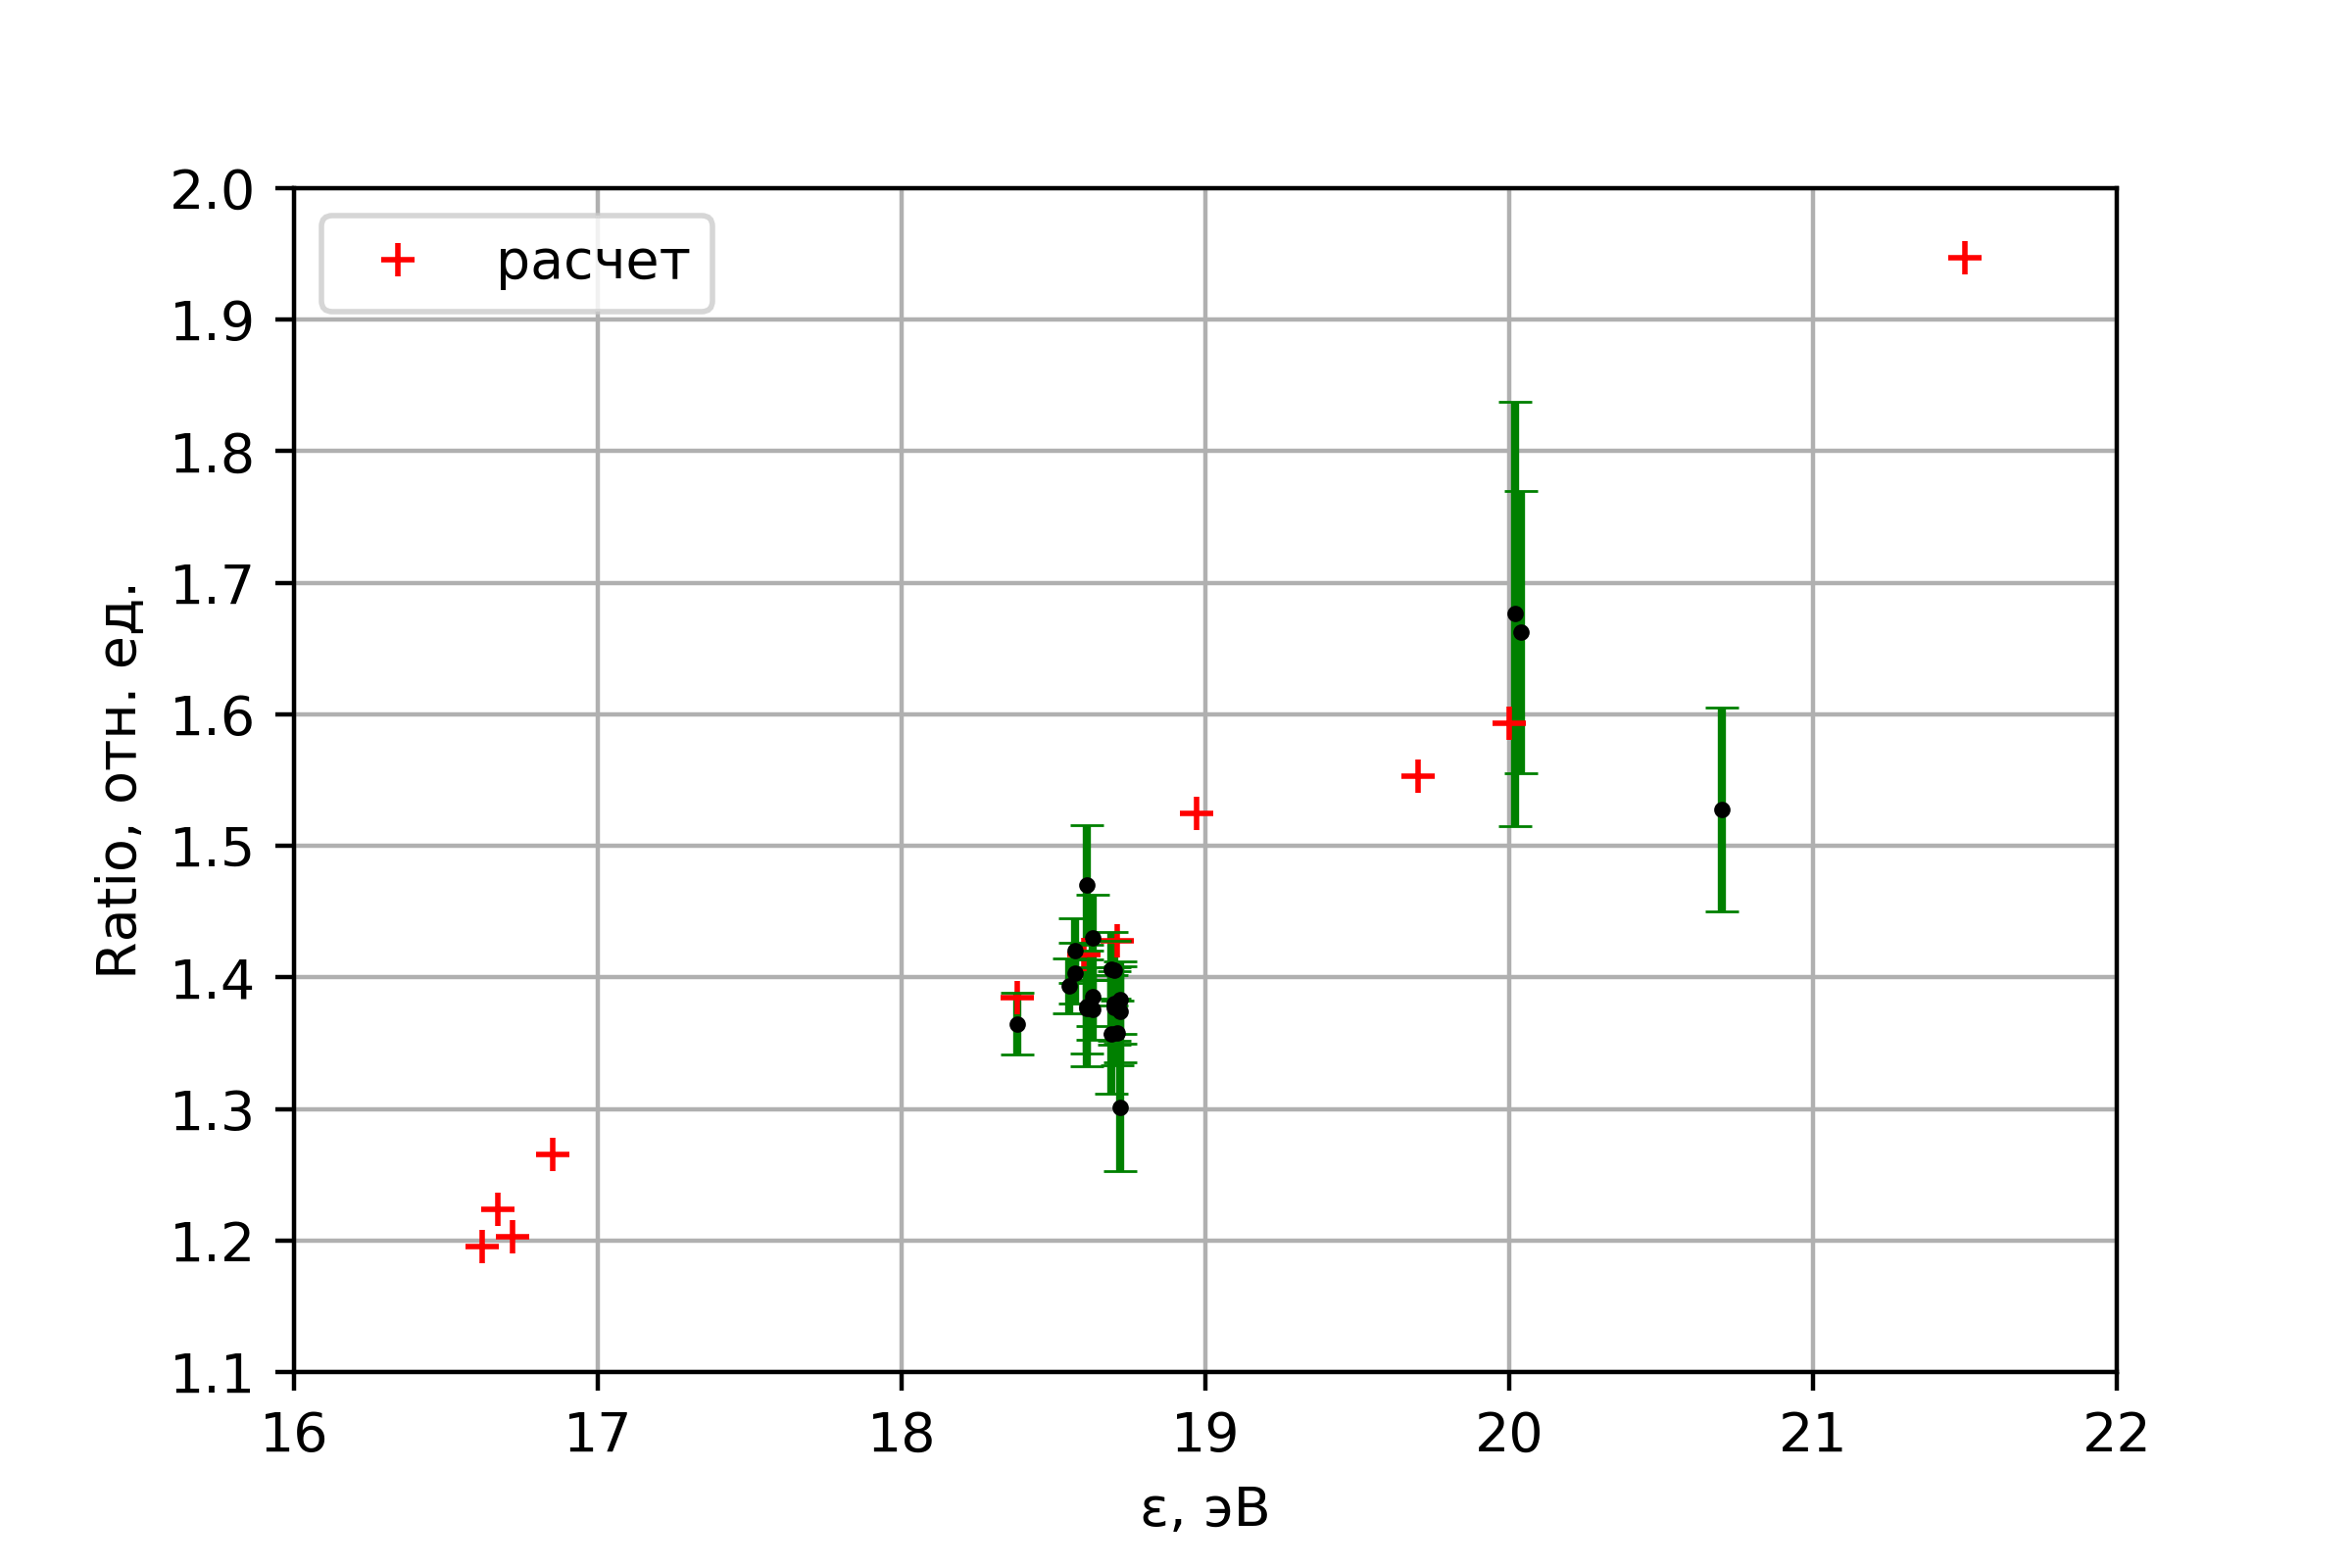
\includegraphics[width=16cm]{figures/Intensities_ratio}
  \caption{Наложены расчетные отношения интенсивностей на рисунок \ref{fig:experimental_ratio}}
  \label{fig:Intensities_ratio}
\end{figure}

Для оценки электронной температуры возмущенного пылевыми частицами положительного столба газового разряда постоянного
тока воспользуемся подходом, описанным в разделе \ref{sec:link_ratio_and_TE}. Для этого необходимо знать, как минимум,
параметры невозмущенного разряда: согласно~\cite{Pustylnik} осевое электрическое поле равняется $E_1 = 2.2$~В/см, а
электронная температура хвостовой части $T_e = 3.2$~эВ \cite{Zobnin2018}. Таким образом, на основе
(\ref{eq:intensities_ratio}) и полученных экспериментальных данных построим невязку $\eta$ с параметризацией значений
осевого электрического поля, которым задается предполагаемая ФРЭЭ возмущенного пылевым облаком газового разряда:
\begin{equation}
    \eta(E_2) = {1 \over N} \sum_{\forall \lambda \in experiment}{|R_{exp}(\lambda) - R_{calc}(\lambda, E_2)| \over {R_{exp}(\lambda) + R_{calc}(\lambda, E_2)}},
\end{equation}
где $E_2$~--~осевое электрическое поле возмущенного пылевыми частицами газового разряда, $R_{calc}$~--~расчетное
отношение интенсивностей, $R_{exp}$~--~отношение интенсивностей, полученное экспериментальным путем, $\lambda$~--~характеристики
спектральных линий, для которых найдено экспериментально отношение интенсивностей, N~--~кол-во таких спектральных линий.

\begin{figure}[t]
  \centering
  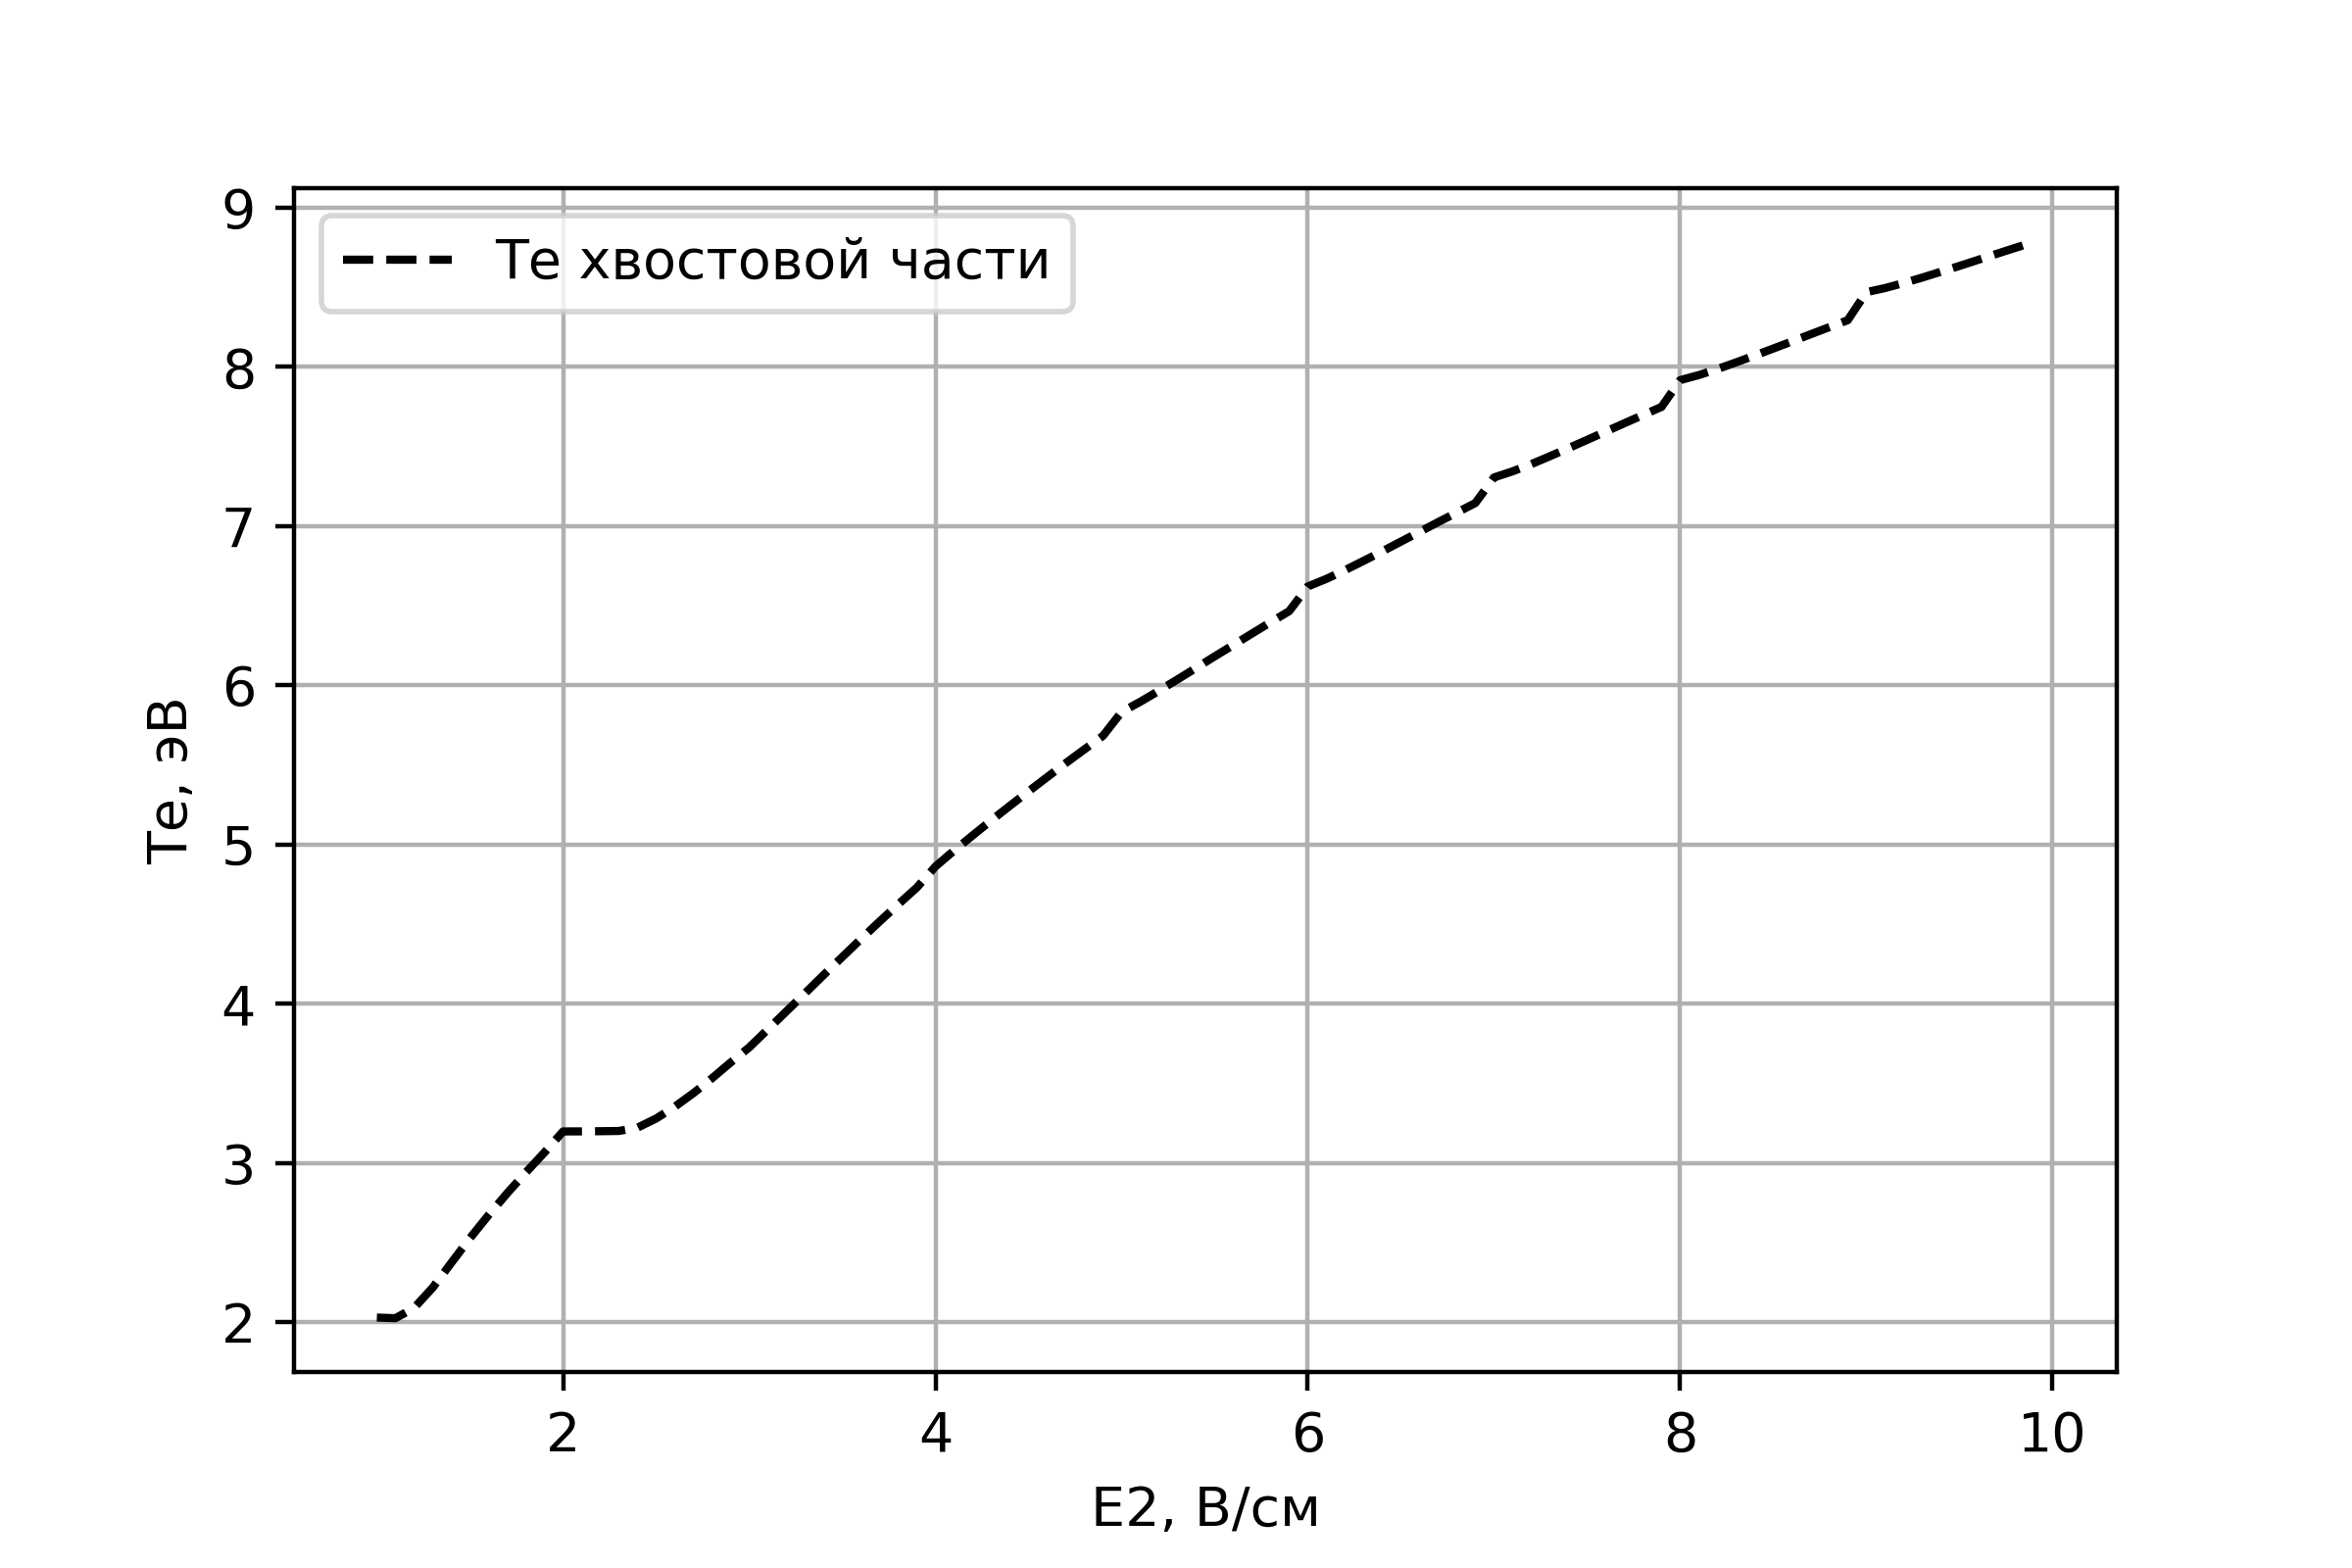
\includegraphics[width=16cm]{figures/Te_tail}
  \caption{Зависимость абсолютных значений расчетной электронной температуры для неупругих электрон-электронных
  взаимодействий от осевого электрического поля, полученных на основе значений параметров невозмущенного разряда $T_e = 3.2$~эВ, $E_z = 2.2$~В/см.}
  \label{fig:Te_tail}
\end{figure}

Полученная невязка имеет четко выраженный минимум при осевом электрическом
поле $E_2 = 2.8$~В/см и значении невязки $\eta = 0.02$ (см.~рисунок~\ref{fig:discrepancy}).
При данном осевом электрическом поле, экспериментальные и расчетные отношения интенсивностей максимально близки друг другу,
что говорит о правильном подборе параметра $E_2$.
Совмещенные результаты экспериментальных отношений с расчетными можно посмотреть на рисунке \ref{fig:Intensities_ratio}.
Из данного графика видно, что расчетная модель довольно хорошо описывает эксперимент. Оценим электронную температуру
согласно (\ref{eq:Te_from_FRE}). Для наглядности построим калибровочную зависимость электронной температуры от
значений осевого электрического поля, используемых для расчета ФРЭЭ (см.~рисунок~\ref{fig:Te_tail}), на основе
параметров невозмущенного разряда. При полученном ранее осевом электрическом поле $E_z = 2.8$~В/см, электронная температура
равна $T_e = 3.5$~эВ.

